\documentclass[11pt]{article}


\usepackage[letterpaper,margin=0.5in]{geometry}
\usepackage{amsmath}
\usepackage{amssymb}
\usepackage{dsfont}
\usepackage{bbm}
\usepackage{stmaryrd}
\usepackage{graphicx}
\usepackage{pbox}
\usepackage{hyperref}
\usepackage{changepage}


\newcommand{\braces}[1]{\left\{#1\right\}}
\newcommand{\abs}[1]{\left|#1\right|}
\renewcommand{\vec}[1]{\mathbf{#1}}
\newcommand{\mean}[1]{\langle #1 \rangle}
\newcommand{\norm}[1]{\left|\left|{#1}\right|\right|}

\newcommand{\beq}{\begin{equation}}
\newcommand{\eeq}{\end{equation}}
\newcommand{\beqa}{\begin{eqnarray}}
\newcommand{\eeqa}{\end{eqnarray}}
\newcommand{\beqaN}{\begin{eqnarray*}}
\newcommand{\eeqaN}{\end{eqnarray*}}

\newcommand{\micron}{\mu\textrm{m}}
\newcommand{\specialcell}[2][c]{%
  \begin{tabular}[#1]{@{}c@{}}#2\end{tabular}}

\newcommand{\boldrho}{\rho\hspace{-5.1pt}\rho}
% \newcommand{\grvec}[1]{#1\hspace{-6pt}#1\hspace{-6pt}#1\hspace{1pt}}
\newcommand{\grvec}[1]{\boldsymbol{#1}}
\newcommand{\one}{\mathds{1}}

\newcommand{\hp}{\circ}%{\odot}%{\circ}
\newcommand{\hd}{\hspace{-1.6mm}\fatslash}%{\oslash}'

\setlength{\parskip}{1em}
\setlength{\parindent}{0in}

\begin{document}

\author{Ahmadreza Ghaffarizadeh \and Samuel H. Friedman \and Shannon M. Mumenthaler \and Paul Macklin${}^*$}
\title{PhysiCell: an open source physics-based multicellular simulator
\break\break
\textbf{\huge{Tutorial}}
}
\date{}
\date{Revision: July 7, 2016}	

\maketitle
This tutorial will teach you how to download, install and run a series of biological problems in PhysiCell.
Please note that this tutorial will be periodically updated.
Users should check \href{http://PhysiCell.MathCancer.org}{PhysiCell.MathCancer.org}  for the latest version. PhysiCell manuscript in preparation for peer review;   
% is currently under review by \textit{PLOS Computational Biology} journal; 
please see the the citation information below.

\section{Citing PhysiCell}
If you use PhysiCell in your project, please cite PhysiCell and the version  number, such as below:\\

\begin{adjustwidth}{2.5em}{0pt}
\textit{We solved the diffusion equations using PhysiCell (Version 1.0.0) [1]}

\indent [1] A Ghaffarizadeh, SH Friedman, SM Mumenthaler, and P Macklin, PhysiCell: an Open Source Physics-Based Cell Simulator for Multicellular Systems, 2016 (in preparation). 

Because PhysiCell extensively uses BioFVM, we suggest you also cite BioFVM as below:

\textit{We implemented and solved the model using PhysiCell (Version 1.0.0) [1], with BioFVM [2] to solve the transport equations.}

\indent [1] A Ghaffarizadeh, SH Friedman, SM Mumenthaler, and P Macklin, PhysiCell: an Open Source Physics-Based Cell Simulator for Multicellular Systems, 2016 (in preparation).

\indent [2] A Ghaffarizadeh, SH Friedman, and P Macklin, BioFVM: an efficient parallelized diffusive transport solver for 3-D biological simulations, Bioinformatics 32(8): 1256-8, 2016. DOI: 10.1093/bioinformatics/btv730
\end{adjustwidth}


\section{Preparing to use PhysiCell}
\subsection{Downloading PhysiCell}
BioFVM is available at \href{http://PhysiCell.MathCancer.org}{PhysiCell.MathCancer.org} and at \href{http://PhysiCell.sf.net}{PhysiCell.sf.net}.
Because we aim for cross-platform compatibility and simplicity, we designed PhysiCell
to minimize external dependencies.  As of Version 1.0, PhysiCell doesn't directly need any external library, however, since PhysiCell is built on the top of BioFVM, pugixml is needed for compiling the code (included in the download).

\subsection{Supported platforms}
PhysiCell should successfully compile and run on any C++11 or later compiler that supports OpenMP.
We recommend using a 64-bit compiler for best results. We target g++ (Version 4.8.4 or later)
on Linux and OSX, and MinGW-W64(gcc version 4.9.0 or later) on Windows for this version (testing and support are planned
for the Intel C++ compiler in the future versions).

\subsection{Including PhysiCell in a project}
\label{including_PhysiCell}
PhysiCell does not require any form of installation for use in a project. Instead, extract all
its cpp and h files in your project directory. All PhysiCell source files begin with the prefix
``\verb:PhysiCell_:''. If your project uses makefiles, you'll want to include
the following lines:

\begin{verbatim}
CC     := g++       # replace with your compiler
ARCH := core2 # a reasonably safe default for most CPUs since 2007
# ARCH := corei7
# ARCH := corei7-avx # earlier i7
# ARCH := core-avx-i # i7 ivy bridge or newer
# ARCH := core-avx2 # i7 with Haswell or newer
# ARCH := nehalem
# ARCH := westmere
# ARCH := sandybridge
# ARCH := ivybridge
# ARCH := haswell
# ARCH := broadwell
# ARCH := bonnell
# ARCH := silvermont
# ARCH := nocona #64-bit pentium 4 or later

CFLAGS := -march=$(ARCH) -O3 -s -fomit-frame-pointer -mfpmath=both -fopenmp -m64 -std=c++11
# replace CFLAGS as you see necessary, but make sure to use -std=c++11 -fopenmp

BioFVM_OBJECTS := BioFVM_vector.o BioFVM_matlab.o BioFVM_utilities.o BioFVM_mesh.o \
BioFVM_microenvironment.o BioFVM_solvers.o BioFVM_basic_agent.o \
BioFVM_agent_container.o BioFVM_MultiCellDS.o

PhysiCell_OBJECTS := PhysiCell_cell_container.o PhysiCell_cell.o PhysiCell_standard_models.o \
PhysiCell_digital_cell_line.o PhysiCell_utilities.o

pugixml_OBJECTS := pugixml.o

COMPILE_COMMAND := $(CC) $(CFLAGS)

BioFVM_vector.o: BioFVM_vector.cpp
	$(COMPILE_COMMAND) -c BioFVM_vector.cpp

BioFVM_agent_container.o: BioFVM_agent_container.cpp
	$(COMPILE_COMMAND) -c BioFVM_agent_container.cpp
	
BioFVM_mesh.o: BioFVM_mesh.cpp
	$(COMPILE_COMMAND) -c BioFVM_mesh.cpp

BioFVM_microenvironment.o: BioFVM_microenvironment.cpp
	$(COMPILE_COMMAND) -c BioFVM_microenvironment.cpp

BioFVM_solvers.o: BioFVM_solvers.cpp
	$(COMPILE_COMMAND) -c BioFVM_solvers.cpp

BioFVM_utilities.o: BioFVM_utilities.cpp
	$(COMPILE_COMMAND) -c BioFVM_utilities.cpp
	
BioFVM_basic_agent.o: BioFVM_basic_agent.cpp
	$(COMPILE_COMMAND) -c BioFVM_basic_agent.cpp
	
BioFVM_matlab.o: BioFVM_matlab.cpp
	$(COMPILE_COMMAND) -c BioFVM_matlab.cpp

BioFVM_MultiCellDS.o: BioFVM_MultiCellDS.cpp
	$(COMPILE_COMMAND) -c BioFVM_MultiCellDS.cpp

PhysiCell_digital_cell_line.o: PhysiCell_digital_cell_line.cpp
	$(COMPILE_COMMAND) -c PhysiCell_digital_cell_line.cpp

PhysiCell_cell.o: PhysiCell_cell.cpp
	$(COMPILE_COMMAND) -c PhysiCell_cell.cpp

PhysiCell_cell_container.o: PhysiCell_cell_container.cpp
	$(COMPILE_COMMAND) -c PhysiCell_cell_container.cpp
	
PhysiCell_standard_models.o: PhysiCell_standard_models.cpp
	$(COMPILE_COMMAND) -c PhysiCell_standard_models.cpp
	
PhysiCell_utilities.o: PhysiCell_utilities.cpp
	$(COMPILE_COMMAND) -c PhysiCell_utilities.cpp

pugixml.o: pugixml.cpp
	$(COMPILE_COMMAND) -c pugixml.cpp
\end{verbatim}

We have listed the common values the can be used for \verb:ARCH:. Please note that we used core2 as the default
one, however, you need to consider choosing your CPU architecture settings from the list for a better performance.
Your compiler flags will require \verb:-fopenmp: for OpenMP (for parallelization
across processor cores) and \verb:-std=c=++11: (to ensure compatibility with C++11 or
later, and should include \verb:-m64: (to compile
as a 64-bit application with greater memory address space).

More sophisticated IDEs may require additional steps to ``import'' the PhysiCell source; see
your software's user documentation for further details.

\section{Your first PhysiCell application:  a simple multicellular system starting from a single cell}
\label{first_example}
We will now create a basic PhysiCell application that creates a spheroid of cells starting from a single cell
placed in a microenvironment simulated by BioFVM. As mentioned earlier, PhysiCell is built on the top of BioFVM,
so if you are not familiar with creating a BioFVM application, please first read the tutorial on BioFVM here
\url{biofvm.mathcancer.org}.

We create this example using the microenvironment in \verb:tutorial3\_BioFVM: where we
used Dirichlet condition for the boundaries of our microenvironment. Now we are going to place a cell at the center
of this microenvironment and let it grow and divide. The first step in creating any experiment in PhysiCell is to declare
and initialize the \verb:cell_container:: a data structure that extends the \verb:BioFVM_agent_container: and is the backbone of
PhysiCell. We need to provide the voxel size we need for the cell container. We discussed how we set this value in supplementary
material of the PhysiCell paper. Voxel size is set to 30 $\micron$ in this experiment.

\begin{verbatim}
Cell_Container* cell_container = new Cell_Container;
cell_container->initialize(minX, maxX, minY, maxY, minZ, maxZ, voxel_size );
\end{verbatim}

Now we can define the cell we want to place in the microenvironment. However, before creating the cell, we first need to define the cell line
that our cell takes its phenotype from. \verb:PhysiCell_digital_cell_line.cpp: provides some default cell lines that can be
used. We will later describe the essential fields you may want to change to define your own digital cell
line or a specific phenotype within a cell line. We use the two following lines of code to create a sample cell line for
cancer cells:

\begin{verbatim}
Cell_Line cancer;
set_cancer_cell_line_MCF7( cancer );
\end{verbatim}

Each cell line is composed of multiple phenotypes. For this example, we just use the first phenotype of cancer cell line (at index 0). Once we
created our cell line, we need to modify it to make it consistent with the number of substrates we have in our microenvironment.
Specifically, we need to change the secretion rates, uptake rates, and saturation densities of the cell line based on the
substrates in the microenvironment and the type of the cell we are working with. For this example, we have only one substrate (oxygen)
that is uptaken by cells. Our cells in this experiment do not secrete any substrate, so the values for secretion rate and saturation density should be zero.
We set the oxygen uptake rate for the cells to 10 in this example.

\begin{verbatim}
cancer.phenotypes[0].secretion_rates.rates.resize( microenvironment.number_of_densities(), 0.0 );
cancer.phenotypes[0].uptake_rates.rates.resize( microenvironment.number_of_densities(), 0.0 ) ;
cancer.phenotypes[0].saturation_densities.densities.resize(microenvironment.number_of_densities()
                                                                                        , 0.0 );
cancer.phenotypes[0].uptake_rates.rates[0] = 10;
\end{verbatim}

Now if we call display\_information function from our cell line, it provides a summary of the cell line.

\begin{verbatim}
Cell line: MCF7
phenotype 0: viable
phenotype 1: physioxic
phenotype 2: hypoxic
phenotype 3: necrotic
phenotype 4: hypoxic_glycolytic
phenotype 5: physioxic_glycolytic
phenotype 6: normoxic_glycolytic
\end{verbatim}

To create a cell, we use \verb:create_cell: method from \verb:PhysiCell_cell.cpp:
and then assign the position of the cell.

\begin{verbatim}
Cell* pCell = create_cell();
pCell->assign_position(500, 500, 500);
\end{verbatim}

Cells need to have access to the microenvironment they are located in, so we associate the cell with the microenvironment we defined earlier.
We also set the phenotype of the cell based on cell line that we defined earlier.

\begin{verbatim}
pCell->register_microenvironment(&microenvironment);
pCell->set_phenotype(cancer.phenotypes[0]);
\end{verbatim}

Now we need to provide cells with a model that manages their life and death cycle. \verb:Physicell_standard_models: has implemented some known
models including basic KI-67, advanced KI-67, live and dead, and total cell models (see the the main PhysiCell paper for more details).

\begin{verbatim}
pCell->advance_cell_current_phase= ki67_advanced_cycle_model;
\end{verbatim}

We also need to specify at what phase in the cycle model the cell is:

\begin{verbatim}
pCell->phenotype.set_current_phase(PhysiCell_constants::Ki67_negative);
\end{verbatim}

Finally, similar to \verb:basic_agents: in BioFVM, we need to call \verb:set_internal_uptake_constants: for the cells.

\begin{verbatim}
pCell->set_internal_uptake_constants(dt);
\end{verbatim}

To run this experiment, we should call the \verb:update_all_cells: function from the \verb:cell_container:
within the main loop of simulation. Note that we also called \verb:simulate_cell_sources_and_sinks: in the main
loop since our cells are uptaking oxygen.


\begin{verbatim}
double t;
double t_max= 60 * 24 * 3; // 3 days
while( t < t_max )
{
    microenvironment.simulate_bulk_sources_and_sinks( dt );
    microenvironment.simulate_cell_sources_and_sinks( dt );
    microenvironment.simulate_diffusion_decay( dt );
    ((Cell_Container *)microenvironment.agent_container)->update_all_cells(dt);	
    t += dt;
}
microenvironment.write_to_matlab( "final_concentration.mat" );
\end{verbatim}

\verb:PhysiCell_utilities: provides some useful methods to log the output of PhysiCell. The main loop can be modified a bit
to keep the track of the cells:

\begin{verbatim}
double t_output_interval = 60.0; // every 1 hour
double t_next_output_time = 0;
int output_index =0;
BioFVM::RUNTIME_TIC();
BioFVM::TIC();
	
std::ofstream report_file ("report_spheroid.txt");
report_file<<"simulated time\tnum cells\tnum division\tnum death\twall time"<<std::endl;
while( t < t_max )
{
    if(  fabs( t - t_next_output_time ) < 0.0001 )
    {
        log_output(t, output_index, microenvironment, report_file);
        t_next_output_time += t_output_interval;						
    }
    microenvironment.simulate_cell_sources_and_sinks( dt );
    microenvironment.simulate_diffusion_decay( dt );
    ((Cell_Container *)microenvironment.agent_container)->update_all_cells(t, 
                                                    cell_cycle_dt, mechanics_dt);		
    t += dt;
    output_index++;
}
log_output(t, output_index, microenvironment, report_file);
report_file.close();
\end{verbatim}

The above code keeps the record of the simulation time, number of cells removed from the system (death),
number of cells that divided, total number of cells, and wall time at each iteration (logged in report.txt).
It also records the detailed description of each cell in \verb:output: folder at each output interval.

To compile and run this example, add the following line to the makefile (if it is not already there):

\begin{verbatim}
physicell_example1: $(pugixml_OBJECTS) $(BioFVM_OBJECTS) $(PhysiCell_OBJECTS) $(UTILITY_OBJECTS) 
    <your_file_name> $(COMPILE_COMMAND) -o PhysiCell_example1 $(BioFVM_OBJECTS)
    $(PhysiCell_OBJECTS) $(UTILITY_OBJECTS) $(pugixml_OBJECTS) <your_file_name>
\end{verbatim}

Then in the command line (or terminal in Unix based systems) type \verb:make physicell_example1:. This will create
an executable file that you can run on your system. 

As listed in Table XXXXXXX of supplementary materials, each cell has a set of function pointers that are set
to default function pointers. There are some other function pointers that are left to users to set. We used one
of these functions in the above experiment: \verb:advance_cell_current_phase:. Use of the function pointers make it easy to
disable a behavior that we are not interested in for an experiment. For example, if in the above experiment, we
want our cells to not move, we can set \verb:pCell->update_velocity: to \verb:do_nothing:; or as another example,
if we do not want our cells to update their volume, we can easily set it by:

\begin{verbatim}
pCell->update_volume = do_nothing;
\end{verbatim}

The source code for this example is provided in \verb:examples/tutorial1_PhysiCell.cpp:.


\section{Example 2: cells growing inside a duct}

Ductal Carcinoma \textit{in situ} (DCIS) is one of the most well-studied types of cancer that starts within ducts of breast. In this
example we show how you can create a simulation of DCIS using PhysiCell. Most part of this example is similar to what we did in previous section. 
The main difference is that in this example, we need to impose the duct structure. All we need to do is to crete a function that returns the distance $d$
of a cell (passed as a pointer) to the duct walls and assign it to the \verb:distance_to_membrane: function pointer of the cells. We use a level set function (a signed distance function d(x)) to represent the breast duct. In this method, $d < 0$ indicates that the cell is inside the duct, $d = 0$ indicates that the cell is on the duct wall, and $d > 0$ indicated that the cell is located outside the duct (in the stroma), $|d|$ is the distance to the duct wall, and $\nabla d(x)$ points outward from the duct wall, oriented from the closest point on the duct wall to the cell. See \ref{Macklin2006Improved} for further details.

The following function implements the level set function we discussed for the duct shown in Figure~\ref{fig:duct_structure}. The code first checks if the cell located inside the cap of the duct (within the semi-sphere) or within the cylinder part of the duct. Based on the result of the test, code executes instruction either at PART1 or PART2 (see the code below). PART1 first computes the distance of the cell from the x-axis, sets the displacement vector accordingly, and returns the distance of the cell from the wall as the difference of duct radius and the distance to x-axis. If the cell is inside the cap of the duct, PART2 computes the distance of the cell to the origin, sets the displacement vector accordingly, and returns the distance of the cell from the cap walls as the difference of semi-sphere radius (same as the duct radius) and the distance to the origin.

\begin{figure}[h]
\centering
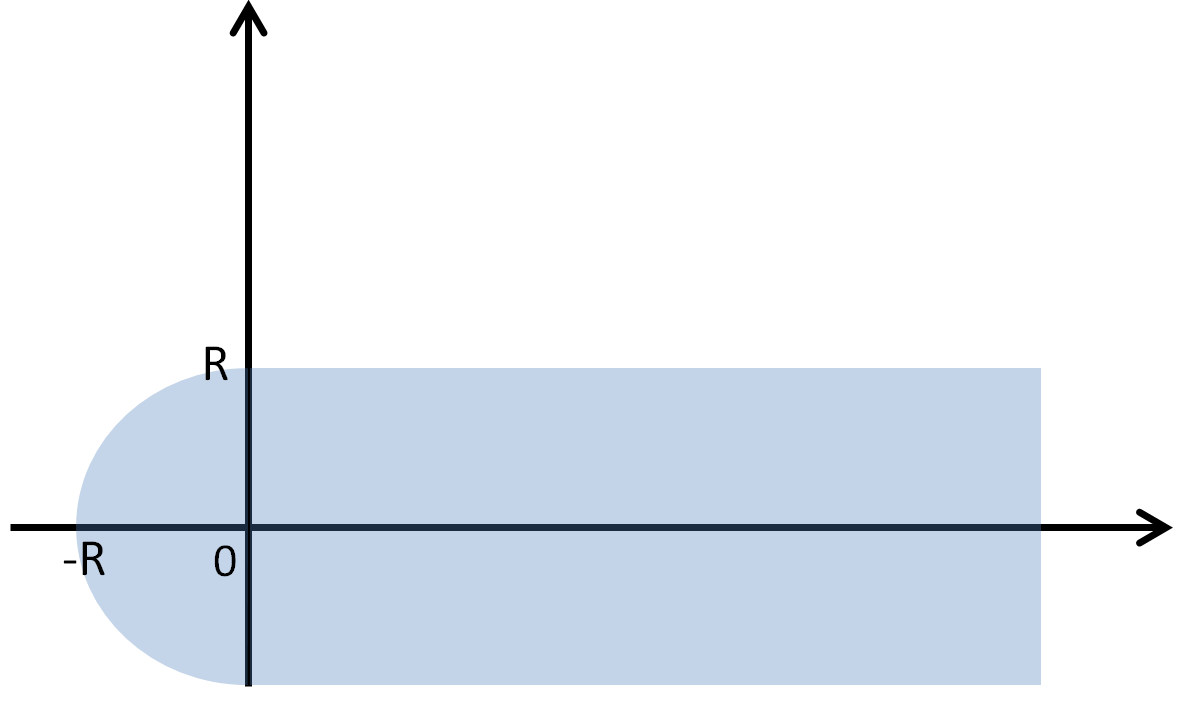
\includegraphics[width=0.5\textwidth]{./images/duct_structure.png} 
\caption{ The duct cross-section at z = 0.  }
\label{fig:duct_structure}
\end{figure}


\textbf{NOTE: any method that is assigned to the} \verb:distance_to_membrane: \textbf{function pointer of the cells must set the displacement vector in addition to returning the distance of the cell from the membrane.}

\begin{verbatim}
double distance_to_membrane_duct(Cell* pCell)
{
    //Note that this function assumes that duct cap center is located at <0, 0, 0>
    double epsillon= 1e-7;
    if(pCell->position[0]>=0) // Cell is within the cylinder part of the duct
    {
        */ ######################### PART1 #########################*/
        double distance_to_x_axis= sqrt(pCell->position[1]* pCell->position[1] + 
                                            pCell->position[2]*pCell->position[2]);
        distance_to_x_axis = max(distance_to_x_axis, epsillon);		// prevents division by zero
        pCell->displacement[0]=0;
        pCell->displacement[1]= -pCell->position[1]/ distance_to_x_axis;
        pCell->displacement[2]= -pCell->position[2]/ distance_to_x_axis;
        return fabs(duct_radius- distance_to_x_axis);
    }

    // Cell is inside the cap of the duct
    */ ######################### PART2 #########################*/
    double distance_to_origin= dist(pCell->position, {0.0,0.0,0.0});  // distance to the origin
    distance_to_origin = max(distance_to_origin, epsillon);			  // prevents division by zero
    pCell->displacement[0]= -pCell->position[0]/ distance_to_origin;
    pCell->displacement[1]= -pCell->position[1]/ distance_to_origin;
    pCell->displacement[2]= -pCell->position[2]/ distance_to_origin;
    return fabs(duct_radius- distance_to_origin);
}
\end{verbatim}

Once the function is implemented, you can assign it to \verb:distance_to_membrane: when you are initializing the cells (see the initiation phase in the previous example). 

\begin{verbatim}
pCell->distance_to_membrane= distance_to_membrane_duct;
\end{verbatim}

The rest of the code is similar to the previous example. This example is very similar to the DCIS simulation we have presented in the paper. If you start with 1000 cells and let the simulation run for about 30 days (about 16 hours on a quad-core machine with hyperthreading), and visualize the output, it should generate something similar to Figure~\ref{xxx} in the paper.

The source code for this example is provided in \verb:examples/tutorial2_PhysiCell.cpp:.


\section{Visualizing outputs}
\label{visualzing_output}
PhysiCell stores its output in two formats: txt and pov. The txt format file at each time step has all the needed information that can be used later for continuing the simulation from that point. For each cell in the txt file, PhysiCell stores cell ID, cell position, cell volume and all subvolumes, cell phase ID, and the elapsed time in the current phase. The pov file is the ready-to-render file that can be rendered using POV-Ray software (download for free from \url{http://www.povray.org/download/}). Please note that the PhysiCell needs \verb:header.inc: and \verb:footer.inc: for rendering the output pov files. The default files are available in XXXX folder of ant PhysiCell download. \verb:header.inc: keeps the information related to the position of camera, the direction of the camera, sources of light, and the color of each cell phase. You may need to manually change this file to get the desired rendering.

We also have provided a Matlab script file that can read a txt format file and create a cross-section of the system. This script can be found at XXXXXX. Note that this script does not rewrite \verb:header.inc: and \verb:footer.inc: files, so you need to have them from the PhysiCell output. 

Please note that the microenvironment can be visualized using BioFVM Matlab functions available in any BioFVM download. 


\end{document} 